\chapter{Introduction}
\section{Motivation}
Sparse LU decomposition has been widely used to solve sparse linear systems of equations found in many scientific
and engineering applications, such as circuit simulation, power system modeling and computer vision.
Applications such as circuit simulation typically requires several thousand iterations
of solving the linear system at different simulation steps. Hence the
solving the sparse linear system is one of the most critical steps in circuit simulation.
However it is a computationally expensive and difficult to parallelize on the traditional
processing systems due to the highly sparse and instance dependent nature of the data which causes sparse 
algorithms to spend significant time data handling.\\
Naturally, an extensive research has been conducted on expediting the sparse LU 
decomposition process for range of computing platforms including the FPGA based systems.
With the recent advancements in the fields of FPGA many researchers have developed 
accelerated solutions for specific scientific applications where matrices are 
symmetric and are diagonally dominant. Such problems are relatively easy to solve and parallelize. 
But in many applications including non-linear time domain circuit simulation, 
matrices do not follow a particular patterns. However such applications
can leverage the fact that the underlying matrix structure, that is the locations of the non-zero elements,
remains same for many iterations and only the numerical values are different in each iteration hence the
data manipulation steps also remains the same. Overall performance can be 
boosted by sharing this manipulation steps. Such methods are already being used 
in many specialized libraries, like KLU (a direct sparse solver for circuit simulation problems).
These methods can leverage further more by parallelizing a large number computation tasks 
using an FPGA.
\section{The Project}

\begin{figure}
    \centering
    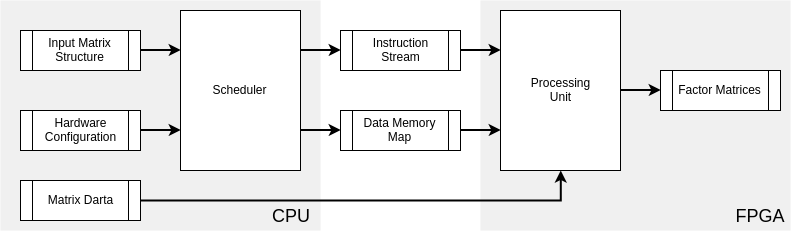
\includegraphics[width = 0.9\linewidth]{./Introduction/projectOverView.png}
    \caption{The overall flow of the project}
    \label{fig:Intro:flow}
\end{figure}

The central goal of the project is to implement a scalable LU solver of the sparse matrices,
especially the asymmetric matrices which arise in circuit simulation problems. The 
project is dived in two major sections: The scheduler and the hardware.\\
The scheduler C++ tool which accepts the target circuit matrix and generates the 
execution schedule based on the location of non-zero elements in the matrix. The 
schedule generated then can be converted into hardware instructions along with 
matrix data. Since the generated schedule does not depend on the actual values, 
it can be used to solve subsequent simulation stages. \\
The hardware processor is a set of deeply pipelined floating point multiply and accumulate (MAC)
, divider units and on-chip block memory units (BRAM). Form here on the collection
of MAC units and divider units is refereed as Processing Elements (PE). The number of
BRAMs and PEs is configurable and can be adjusted according to the need and available
FPGA resources. the hardware accepts the data and instruction set generated 
from the scheduler tool to find the values of the factor matrices. \\
This report is divided in three major sections:
\begin{itemize}
    \item Preliminaries and literature review: \ref{chapter:litRev}, \ref{figure:theory}
    \item Implementation
    \item Testing methodology and results
\end{itemize} 


% \begin{figure}[h]
%     \centering
%     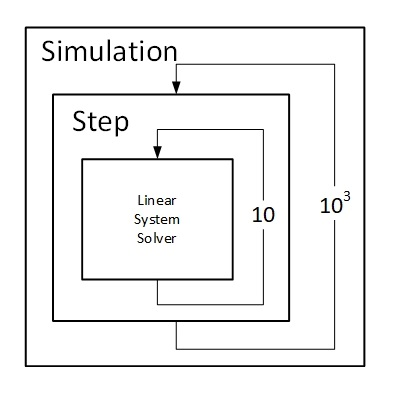
\includegraphics[width = 0.4\textwidth]{./Introduction/motive.jpg}
%     \caption{Circuit simulations typically requires several thousand solves of structurally similar linear systems}
%     \label{fig:Intro:motive}
% \end{figure}
